\documentclass[conference]{IEEEtran}
\IEEEoverridecommandlockouts
% The preceding line is only needed to identify funding in the first footnote. If that is unneeded, please comment it out.
\usepackage{url}
\usepackage{cite}
\usepackage{amsmath,amssymb,amsfonts}
\usepackage{algorithmic}
\usepackage{graphicx}
\usepackage{textcomp}
\usepackage{xcolor}
\def\BibTeX{{\rm B\kern-.05em{\sc i\kern-.025em b}\kern-.08em
    T\kern-.1667em\lower.7ex\hbox{E}\kern-.125emX}}
\begin{document}

\title{An RNN Based Mechanism for File Prefetching \\
%{\footnotesize \textsuperscript{*}Note: Sub-titles are not captured in Xplore and
%should not be used}
%\thanks{This work is supported by the National Key R\&D Program of China (Grant 2017YFB0202201)}
}
%1\textsuperscript{st}
\author{\IEEEauthorblockN{Hui Chen, Enqiang Zhou, Jie Liu, Zhicheng Zhang}
\IEEEauthorblockA{
\textit{School of Computer Science} \\
\textit{National University of Defense Technology} \\
Changsha, China\\
code2hack4ever@gmail.com, eqzhou@nudt.edu.cn}
%\and
%\IEEEauthorblockN{Enqiang Zhou*}
%\IEEEauthorblockA{
%\textit{School of Computer Science} \\
%\textit{National University of Defense Technology} \\
%\textit{name of organization (of Aff.)}\\
%Changsha, China\\
%eqzhou@nudt.edu.cn}
}

\maketitle

\begin{abstract}
Many applications spend a large proportion of the execution time to access files. To narrow the increasing gap between computing and I/O performance, several optimization techniques were adopted, such as data prefetching and data layout optimization. However, the effectiveness of these optimization processes heavily depends on the understanding of the I/O behavior. Traditionally, spatial locality and temporal locality are mainly considered for data prefetching and scheduling policy. Whereas for most real-world workloads, the file access pattern is hard to capture. 

For the goal of deeply and intelligently understanding the I/O access pattern of modern applications, and efficiently optimizing the performance of current file systems, we propose a new mechanism to embed file names to vectors and train a gated recurrent neural network to provide policies for file prefetching and cache replacing.
\end{abstract}

\begin{IEEEkeywords}
    Distributed File System, File Prefetching, Word Embedding, RNN

\end{IEEEkeywords}

\section{Introduction}
Distributed file systems such as HDFS\cite{HDFS}, GlusterFS\cite{GlusterFS}, Ceph\cite{Ceph}, Lustre\cite{Lustre}, etc., have been widely deployed as back-end storage systems for parallel/distributed applications. with the data scale continuously increased, I/O access latency between computing nodes and storage servers has become one of the severest bottlenecks in this big data era. To narrow this performance gap, data caching/prefetching in file systems is one of the most well-known optimization techniques. Caches with high throughput and low latency devices like non-volatile memories(NVMs) and solid-state drives(SSDs) are placed at different levels of the I/O stack to hide network and disk latency.

To cache data from lower storage in a predictable manner, access pattern detection is essential. Traditionally, spatial locality and temporal locality are most generally considered facts. \textit{Readahead} is a basic mechanism implemented by most file systems\cite{WhyDoes} including Linux kernel, which prefetches constant size of data from an opened file to the cache. For workloads executing sequential read, this approach benefits a lot due to the simple and definite pattern. Unfortunately, many applications especially scientific ones usually do not access files sequentially.

The main contributions of this paper can be summarized as follow.
\begin{itemize}
    \item We propose an approach to embed the names of files or directories with Skipgram algorithm, mapping file/directory names to vectors, thus providing a quantitative way to analyze relations among files and directories.
    \item To collect I/O access history, we implement a trace translator into GlusterFS to monitor and trace specific I/O requests.
    \item Base on the embedding mechanism mentioned above, we build a gated recurrent neural network to capture I/O access pattern and encode it with hidden states of the GRU (Gated Neural Unit). We combine the hidden states with file vectors to build a file classifier, which dynamically decides whether a file should be cached or purged from the cache.

\end{itemize}

\section{Related Work}
The I/O subsystem is becoming the bottleneck of high-performance distributed systems, especially there are many communication-intensive applications in them \cite{Related_Network_I/O_load_based}. In order to achieve potential performance enhancements of storage systems, a variety of I/O history analysis-based I/O optimization mechanisms have been proposed previously 
\cite{Related_Multi_Layer_Event_Trace_Analysis} \cite{Related_Towards_an_I/O_tracing_framework_taxonomy} \cite{Related_DiskSeen} \cite{A_Prefetching_Scheme_Related} \cite{Scalable_IO_Tracing_Related}. However, existing approaches including the aforementioned ones have mostly focused on classifying I/O access patterns by analyzing either the history of applications’ I/O requests
\cite{Parallel_IO_Prefetching_Related} \cite{Learning_To_Classify_Related} or the track of block access events \cite{Related_DiskSeen} \cite{A_Prefetching_Scheme_Related}, so that the analyzed results can be used for direct I/O optimization strategies, such as data prefetching. The mechanism of data prefetching focuses on how to forecast future possible read requests, and thus, the accuracy of request prediction is critical to the effectiveness and applicability of data prefetching.

There is a wide range of sophisticated approaches to fulfill data prefetching, which utilize hidden Markov models, neural networks or other predictive algorithms to forecast I/O operations by analyzing I/O access patterns of the application 
\cite{Parallel_IO_Prefetching_Related} \cite{IO_Acceleration_with_Related} \cite{An_Automatic_Prefetching_Related} \cite{Reducing_File_System_Latency_Related} \cite{Automatic_ARIMA_Related}. In summary, these mechanisms employ specific hard-coded algorithms to predict the application's future I/O access requests based on past I/O tracks for prefetching data.

\section{Background and Motivation}
\subsection{Introduction to GlusterFS}
GlusterFS is a scalable distributed filesystem which is suitable for data-intensive workloads such as cloud storage and high-performance computing. It aggregates various storage servers over Ethernet or Infiniband RDMA (Remote Direct Memory Access) interconnect into one large parallel network file system. Servers are typically deployed as storage bricks.

Since version 3.7, the newly implemented feature \textit{tiring} enables different storage types to be used by the same logical volume. As Fig.\ref{fig:tiering} shows, the two types of bricks are classified as \textit{cold} and \textit{hot}. The hot group acts as a cache for the cold group. With fine-tuned prefetching and cache replacing policy, a large proportion of I/O requests are forwarded to the \textit{hot} bricks, thus significantly decreasing access latency. In this case, we can reframe caching/prefetching optimization tasks to binary classification problems, the objective of which is to dynamically decide whether a file is \textit{hot} or \textit{cold}.

\begin{figure}
\centering
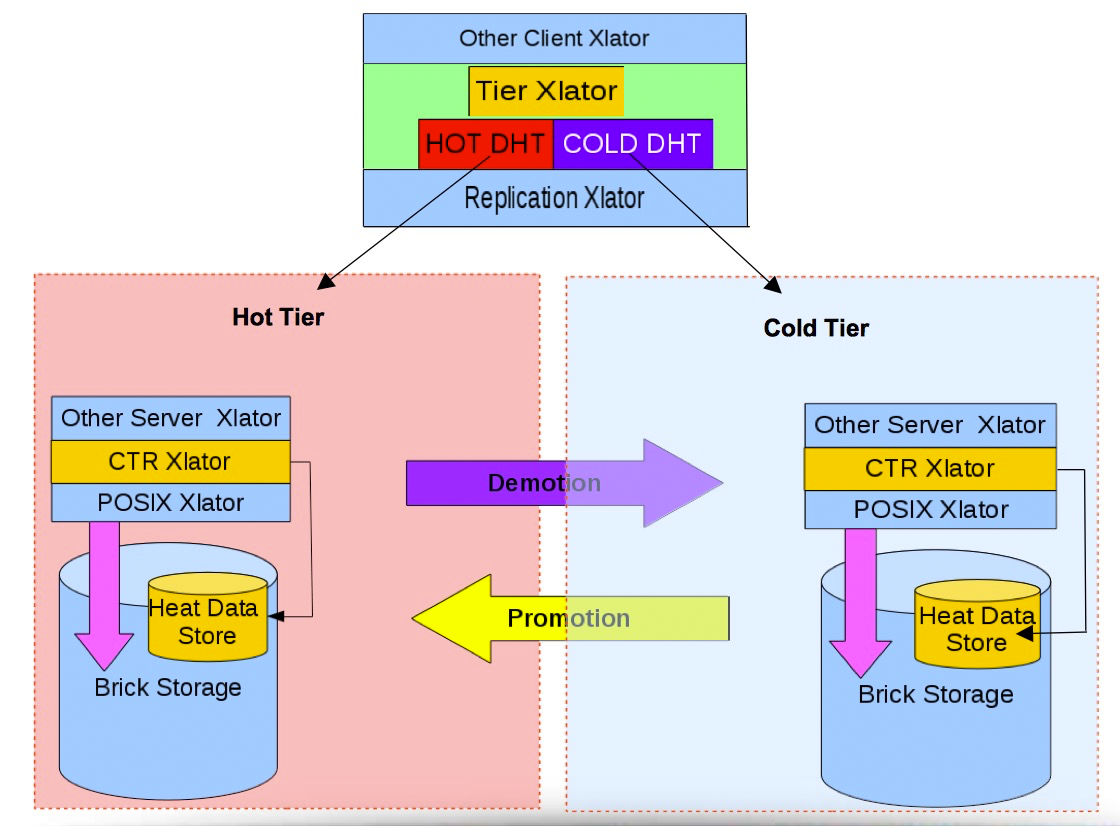
\includegraphics[width=0.5\textwidth]{images/tiering}
\caption{Data tiering in GlusterFS}
\label{fig:tiering}
\end{figure}

\subsection{Word Embedding}
The concept word embedding is a set of language models for distributed representations of words in \textit{Natural Language Processing}(NLP), aiming at mapping natural words to real number vectors based on context provided by specific corpora.
These mapping mechanisms include neural networks, dimensionality reduction on the word co-occurrence matrix, probabilistic methods, etc.

Among the mechanisms mentioned above, the Skip-gram model is an efficient method for learning high-quality distributed vector representations that capture a large number of precise syntactic and semantic word relationships.

%Given a word vocabulary of size $W$, where a word is identified by $w \in {1,\dots,W}$, 
%and a corpus consists of a sequence of words $w_1, \dots, w_T$, the objective of skip-gram algorithm is to maximize the following log probability:
%\begin{equation}
%\frac{1}{T}\sum_{t=1}^{T}\sum_{-c \leq j \leq c,j \neq 0} \log p(w_{t+j} | w_t),
%\end{equation}
%Where $w_t$ denotes the target word at position $t$ in the training corpus and $c$ is the size of context window.
%A basic definition of $p(w_t+j | w_t)$ is the softmax function:
%\begin{equation}
%    p(w_O | w_I) = \frac{ \exp( {v'}_{w_O}^{\top} v_{w_I}) }{\sum_{w=1}^W \exp({v'}_w^{\top} v_{w_I})}
%\end{equation}
%However, it's generally impractical to calculate softmax function due to the tremendous \textbf{(EDIT)}computational complexity,
%as the size of vocabulary may be too large.
%To estimate ...

\subsection{Gated Recurrent Neural Networks}
RNNs(\textit{Recurrent Neural Networks}) have been widely utilized and shown excellent performance in multiple NLP tasks,
such as speech recognition, machine translation, and text emotion classification, etc. The RNN is an extension of a conventional feedforward neural network, which can process a variable-length sequence input. Given a sequence input $x = (x_1, x_2, \dots, x_T)$, the RNN updates its recurrent hidden state $h_t$ by
\begin{equation}
    \mathbf{h_t}=
        \begin{cases}
            0, &t=0 \\
            \phi(\mathbf{h_{t-1}, \mathbf{x_t}}), &\text{otherwise}
        \end{cases}
\end{equation}
Where $\phi$ is a nonlinear function calculating current hidden state $h_t$ based on last state $h_{t-1}$ and current input $x_t$.
\begin{figure}
\centering
\includegraphics[width=0.3\textwidth]{images/GRU_clear}
\caption{Gated recurrent unit}
\end{figure}
The GRU(gated recurrent unit)\cite{GRU} is a gating mechanism in RNNs, which is like an LSTM(Long Short-Term Memory)\cite{LSTM} with forget gate but has fewer parameters.

\section{Design}
\subsection{Path Embedding Model}
Since word embedding mechanisms have significantly promoted the performance of plenty of NLP tasks, we assume that these methodologies are suitable in analytics and optimizations for POSIX (Portable Operating System Interface) file systems as well. \textit{e.g.}, given paths like \textit{/a/b/c/}, \textit{/a/b/d}, we can claim that \textit{a} and \textit{b}, \textit{b} and \textit{c} are parent-child pairs, while \textit{c} and \textit{d} are a pair of brothers with the same parent \textit{b}. Or, intuitively, they are logically close to each other in this directory tree. This basic relation is analogous to 2-Grams model in natural language models.

Formally, given a directory tree accessed by a specific workload such as compiling, it is assumed that the naming conventions and directory structure are regularly formed by producers or users. Thus it is possible to form vocabulary and train an embedding model to represent each filename as a vector.

To generate corpora for training purposes, we recursively traverse the target directory from root entry and print the paths into a text file line by line. After that, the Skip-gram algorithm is invoked to train an embedding model, which finally provides a vocabulary for all the occurred directory/file names and a table consists of vectors for these names.


\subsection{Access Pattern Analytics with Gated Recurrent Neural Network}
\subsubsection{Data Pre-processing}
To collect file access histories, we insert a trace translator into GlusterFS. So far, we mainly focus on file \textit{open} operation to detect when, how and what files does the workload starts to access during its lifetime, attempting to reveal its underlying access patterns beyond the basic locality. The components of the \textit{path} in each \textit{open} request are transformed and added up to form a vector. e.g., given $i$th accessed path named \textit{/foo/bar/file}, the three components are respectively transformed into three vectors: $\{\mathbf{v}_1, \mathbf{v}_2, \mathbf{v}_3\}$, and summed up to form a vector $\mathbf{x}_i = \mathbf{v}_1 + \mathbf{v}_2 + \mathbf{v}_3$. Finally, a sequence of vectors $\mathbf{x}=(\mathbf{x_1}, \dots, \mathbf{x_T})$ representing access history of size $T$ are generated.

\subsubsection{GRU-based Model Building}
In our design, we utilize a single-layer GRU to calculate and update the hidden state, which implicitly represents the access pattern of the target workloads. Given dataset $\mathbf{x} = (\mathbf{x}_1,\dots,\mathbf{x}_T)$ representing a sequence of file access history executed by the target workload, we take these vectors as input sequence for the GRU and train the model. 

At time $t$, the activation $h_t^{(j)}$, which denotes the $j$th element of the hidden state $\mathbf{h}_t$, is a linear interpolation between the previous activation $h_{t-1}^{(j)}$ and the candidate activation $\tilde{h}_t^{(j)}$:
\begin{equation}
    h_t^{(j)} = (1-z_t^{(j)}) h_{t-1}^{(j)} + z_t^{(j)}\tilde{h}_t^{(j)},
\end{equation}
Where $z_t$ is denoted as an \textit{update gate}, calculated by a sigmoid function over input $\mathbf{x_t}$ and previous state $\mathbf{h_{t-1}}$:
\begin{equation}
z_t^{(j)} = \sigma(W_z \mathbf{x}_t + U_z \mathbf{h}_{t-1})^{(j)}
\end{equation}
The candidate activation $\tilde{h}_t^{(j)}$ is computed by:
\begin{equation}
    \tilde{h}_t^{(j)} = \tanh(W \mathbf{x}_t + U (\mathbf{r}_t \odot \mathbf{h}_{t-1}))^{(j)}
\end{equation}
Where $\mathbf{r}_t$ are \textit{reset gates} and $\odot$ is a pointwise multiplication(Hadamard product).
The reset gate is calculated by
\begin{equation}
    r_t^{(j)} = \sigma(W_r \mathbf{x}_t + \mathbf{U}_r \mathbf{h}_{t-1})^{(j)}
\end{equation}
To discriminate files between \textit{hot} and \textit{cold}, our goal is to train the GRU to provide hidden states for classification. We denote $N$ as the approximation of the number of files fit in the cache, thus at time $t$, the following $N$ files(vectors) are labeled as \textit{hot}, i.e., positive samples, while the others are labeled as \textit{cold}(negative). As long as $\mathbf{h}_t$ is calculated, the objective is to maximize the log probability
\begin{equation}
    \label{eq.obj}
    \sum_{i=1}^N \log P(\mathbf{x}_{t+j}|\mathbf{h}_t)
\end{equation}
Where we calculate the probability $P(\mathbf{x}_{t+j}|\mathbf{h}_t)$ by
\begin{equation}
    P(\mathbf{x}_{t+j}|\mathbf{h}_t) = \sigma(\mathbf{x}^\top_t \mathbf{h}_t)
\end{equation}
Thus we obtain the loss function for training
\begin{equation}
    arg\,max L(\theta) = \sum_{i=1}^N \log \sigma(\mathbf{x}^\top_t \mathbf{h}_t)
\end{equation}
Where the parameter $\theta = \{W_z, U_z, W, U, W_r, U_r\}$. We train this GRU with BPTT(Backpropagation Through Time).

\section{Evaluation}
\subsection{Experiment and Parameter Settings}
We use a 4 node cluster to build a distributed file system based on GlusterFS. Each node is deployed on a CentOS7 Server virtual machine on the different physical machines connected by Ethernet and each virtual machine has one CPU, 1G memory and 20G RAM. Each node is equipped with a hard disk as \textit{cold} brick, and an SSD with a volume of 40 GB deployed as the \textit{hot} brick.

We choose compiling workloads as the target and collect 20 different repositories from Github. We split these repositories into two groups, 10 arbitrary repositories for training and the others for testing. 

To evaluate the performance of our model, we adjust the context window size $N$ for testing. Whereas another hyperparameter, the dimension of the embedded vectors is fixed to be 16. 
\subsection{Results for Hit Rate and Access Latency Testing}

\begin{table}[htbp]
    \caption{Results for hit rate and access latency testing} 
\begin{center}
    \begin{tabular}{ |c|c|c| } 
     \hline
     \textbf{\textit{Size of}}&\textbf{\textit{Average}} &\textbf{\textit{Average Access}}\\ 
     \textbf{\textit{Context Window}}& \textbf{\textit{Hit Rate}} & \textbf{\textit{Latency(ms)}}\\
     \hline
     \hline
     0	&0	&270\\
     \hline
     50	&0.13	&263\\
     \hline
     100	&0.21	&255\\
     \hline
     150	&0.26	&242\\
     \hline
     200	&0.42	&233\\
     \hline
     250	&0.53	&225\\
     \hline
     300	&0.66	&221\\
     \hline
     350	&0.77	&207\\
     \hline
     400	&0.74	&218\\
     \hline
     450	&0.7	&231\\
     \hline
     500	&0.67	&245\\
     \hline
    \end{tabular}
\end{center}

%    The first line of data refer to the baseline, where the size of context window is set to 0, 
%    that means our prefetching mechanism does not work.}
    \label{table:result}
\end{table}
As shown in Table. \ref{table:result}, where the first line of data refers to the baseline, i.e., the model and the prefetching mechanism do not work. We can conclude that our mechanism brings benifits to the file system compared to the non-prefetching state. From Fig.~\ref{fig:hit_rate} and Fig.~\ref{fig:latency}, we can observe that this profit brought by our mechanism is limited, due to the increasing tradeoff when the context window is enlarging.
\begin{figure}
\centering
\includegraphics[width=.5\textwidth]{images/hit_rate}
\caption{Hit rate testing}
\label{fig:hit_rate}
\end{figure}

\begin{figure}
\centering
\includegraphics[width=.5\textwidth]{images/latency}
\caption{Access latency testing}
\label{fig:latency}
\end{figure}
%\subsection{\textcolor{red}{EDIT}Similarity Experiment for Directory/File Names}
%In this part, we picked up \textcolor{red}{edit} most frequently occured names from vocabulary, which is generated from the training group of repositories with Skip-gram algorithm.
%We utilize PCA(\textit{Principal Component Analysis}) to project these \textcolor{red}{edit} vectors(\textcolor{red}{EDIT}) into a 2-D graph.
%As fig(\textbf{refhere}) illustrates, 

%\subsection{\textcolor{red}{edit}{Evaluation for dynamically file classification}}
\section{Conclusion}
In this paper, we systematically discuss the similarity between natural language processing and POSIX file systems, and propose a new approach to represent POSIX file/directory names with the Skip-gram algorithm. With this embedding mechanism, we map the file/directory names into a high dimension vector space, where the relation between files can be depicted by the dot production of these two vectors.  

Based on this embedding mechanism, we exploit a single-layer GRNN(Gated Recurrent Neural Network) taking file access history as sequence input. With well trained GRU, we can encode the access pattern to the hidden state and dynamically decide whether a file is \textit{hot} or \textit{cold}, thus providing hints for caching/prefetching and cache replacing policies.

There are several works to accomplish in the future. First, the size of the context window should be adaptive to the volume of the cache, as well as the CPU resources of the storage nodes. Also, our work should be scaled to serve more real-world workloads rather than single-process applications like compiling, especially for scientific workloads in exascale parallel computing and cloud computing circumstances.
\section{Acknowledgments}
Supported by the National Key Research and Development Program (Grant NO. 2017YFB0202201).
\bibliographystyle{plain}
\bibliography{paper}

\end{document}